\documentclass[10pt,a4paper]{article}
\usepackage[spanish,es-noshorthands]{babel}
\usepackage[utf8]{inputenc}
\usepackage[T1]{fontenc}
\usepackage{lmodern}
\usepackage[margin=1.8cm,top=1.5cm,bottom=1.7cm]{geometry}
\usepackage{graphicx}
\usepackage{booktabs}
\usepackage{tabularx}
\usepackage{amsmath}
\usepackage{xcolor}
\usepackage{enumitem}
\usepackage{caption}
\usepackage{tikz}
\usetikzlibrary{arrows.meta,positioning}
\usepackage[hidelinks]{hyperref}

\definecolor{azul}{HTML}{2E6DB4}
\definecolor{rojo}{HTML}{B3441F}
\definecolor{verde}{HTML}{6FAE3C}
\definecolor{morado}{HTML}{8B5BB5}
\definecolor{gris}{HTML}{7A7A7A}

\captionsetup{font=small,labelfont=bf,skip=3pt}
\setlist{nosep,leftmargin=*}
\setlength{\parskip}{3pt}
\setlength{\parindent}{0pt}
\setlength{\textfloatsep}{8pt}
\setlength{\intextsep}{6pt}

\begin{document}

\begin{center}
{\Large\bfseries Proyecto Integrador 2. Avance y propuesta de grafos y recomendación}\\[3pt]
{\small Ricardo Acuña, Juan Aquino y Camilo Soto. Minería de Datos Masivos, 2026 2. Prof. Heider Sanchez.}\\[1pt]
{\small Fuente: Contrataciones Abiertas del Perú, estándar OCDS, OECE, licencia CC BY 4.0, paquetes 2023 a 2025 descargados el 26/10/2026.}
\end{center}

\textbf{De qué trata.} El proyecto 1 describió el gasto proceso por proceso; este mira \textbf{relaciones}: quién le compra a quién y quién compite con quién. Las Partes I y II están cerradas. Para la Parte III y la Parte IV se presenta la propuesta de sistemas de recomendación y de grafos sobre los que se aplicará PageRank, HITS y un grafo KNN. Todo hallazgo se presenta como señal descriptiva para priorizar una revisión, nunca como acusación.

%==========================================================================
\section*{Parte I. Base relacional en Spark}

Toda la parte corre en Spark (modo local, 2 GB y 3 hilos). Parte de la tabla limpia del proyecto 1 y produce los tres objetos que piden las demás partes, exportados en Parquet.

\textbf{1. Resolución de entidades.} El mismo proveedor aparece con varios identificadores, sobre todo los consorcios, que reciben un código nuevo por cada inscripción. Primero se unen claves exactas (RUC y nombre normalizado) y luego se hace una pasada difusa con \textbf{MinHash y LSH propios} en DataFrames, 10 bandas de 4 filas, porque el MinHashLSH de MLlib no terminaba sobre nombres que comparten la palabra CONSORCIO. Una regla de validación evita fusiones falsas: dos códigos que compiten en el mismo proceso son, por definición, distintos. Resultado: de 209.207 identificadores quedan \textbf{165.615 proveedores reales}, y la reducción vive casi entera en los consorcios, 103.722 códigos que son 60.776 consorcios (figura~\ref{fig:p1}, izquierda).

\textbf{2. Los tres artefactos.}
\begin{enumerate}
\item \textbf{Vectores de características}: 62.462 proveedores y 2.968 entidades, con escala, alcance, dependencia y competencia.
\item \textbf{Matrices de interacción}: entidad por proveedor, 2.964 por 62.462 con densidad de 0,06 \%, y entidad por familia CUBSO, 2.954 por 368 con 3,2 \%. La señal es implícita: número de adjudicaciones y monto, por año.
\item \textbf{Grafo de coparticipación de proveedores}: dos proveedores se unen si se presentaron al mismo proceso. Se prefirió al grafo KNN porque aquí la relación existe en el dato. Dos decisiones lo hacen informativo: se descartan procesos con más de 50 participantes, porque uno de 300 genera 44.850 pares que no son relación, y cada coincidencia pesa $1/(n-1)$ (peso de Newman). Se exigen al menos 2 procesos compartidos, el criterio que más reduce aristas según el barrido de sensibilidad. Queda en \textbf{70.383 nodos y 2,50 millones de aristas}, con 97,4 \% en la componente gigante y grado medio de 71.
\end{enumerate}

\textbf{3. Particionado.} La tabla de hechos se escribe con partitionBy por año, y un filtro por año se vuelve PartitionFilter, sin abrir los otros años. El autojoin por proceso que arma el grafo es el paso más caro; se midió su tiempo según particiones de barajado y se fijaron 8, con ejecución adaptativa activa.

\begin{figure}[h]
\centering
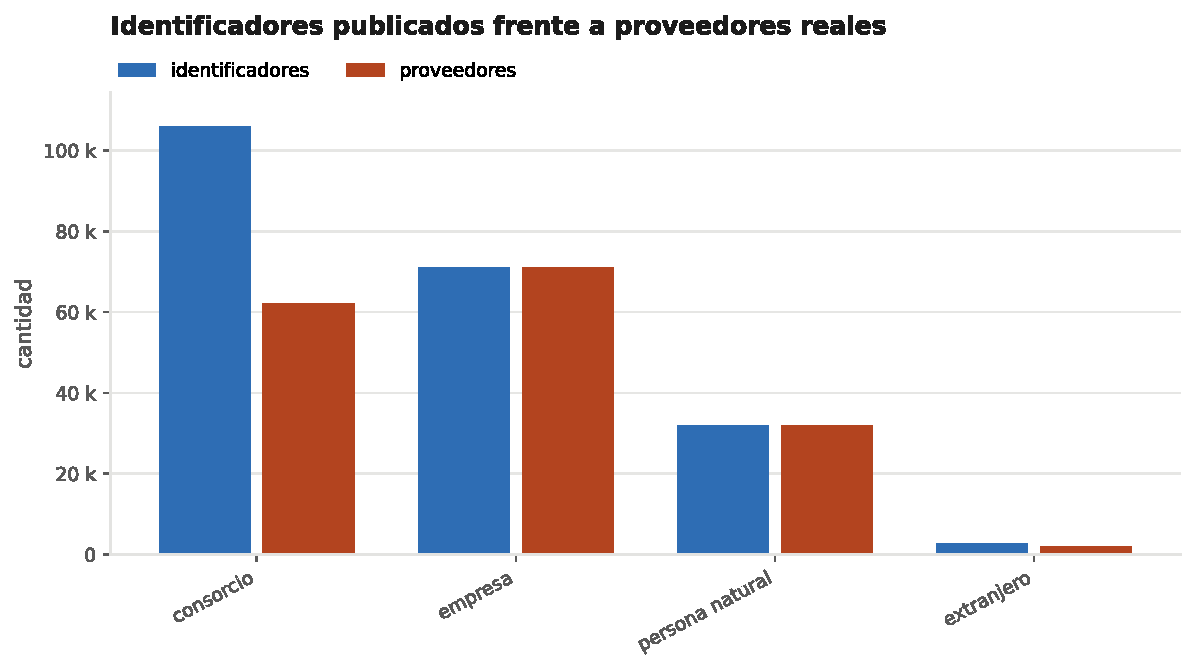
\includegraphics[height=4.6cm]{figs/f02_resolucion.pdf}\hfill
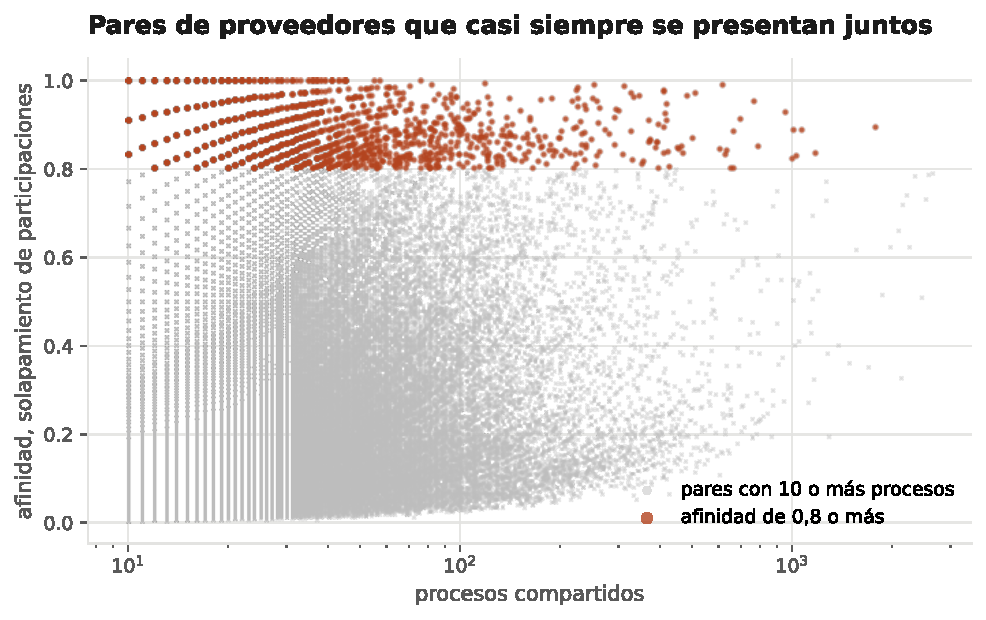
\includegraphics[height=4.6cm]{figs/f07_afinidad_pares.pdf}
\caption{Izquierda: identificadores publicados frente a proveedores reales tras la resolución. Derecha: afinidad de pares con 10 o más procesos compartidos; en rojo, 4.847 pares que coinciden en el 80 \% o más de las participaciones del menos activo.}
\label{fig:p1}
\end{figure}

\textbf{Hallazgos de la Parte I.} Solo el 26 \% de las relaciones entidad y proveedor de 2025 ya existía en 2023 o 2024: la relación nueva es la norma, lo que motiva la Parte III. Y ordenar pares por conteo de coincidencias solo encuentra a los participantes masivos; medido como \textbf{afinidad} (procesos compartidos entre las participaciones del menos activo) aparecen 4.847 pares que se presentan juntos casi siempre, una cola de revisión para el área de competencia.

%==========================================================================
\section*{Parte II. Clustering y detección de anomalías}

\textbf{Población y rasgos.} Proveedores con al menos tres adjudicaciones, 12.062, porque con una sola adjudicación las tasas valen 0 o 1 y el algoritmo encuentra esquinas del cubo y no perfiles. Doce rasgos en cuatro grupos: escala (adjudicaciones, monto total y mediano, en logaritmo), alcance (entidades, departamentos, familias), dependencia y continuidad (cuota del mayor cliente, meses activos) y competencia y rubro (tasa de victoria, postor único, sin concurso, obras). Se estandarizan y se aplica \textbf{PCA} en MLlib: la primera componente explica solo el 40 \% y hacen falta 6 para el 90 \%, así que el comportamiento no se reduce al tamaño.

\textbf{Métodos, propios y contrastados con bibliotecas.}
\begin{enumerate}
\item \textbf{KMeans++}: el codo del SSE sugiere $k=5$, pero la silueta es máxima en $k=4$ (0,387) y se adopta ese; se valida contra KMeans de MLlib.
\item \textbf{Jerárquico de Ward} sobre una muestra: cortado en 4 grupos coincide con KMeans con ARI de 0,62, una confirmación por un camino independiente.
\item \textbf{DBSCAN}: min\_pts igual a 12, el doble de la dimensión, y eps de 1,31 leído en el codo de la curva de distancia al vecino 12; marca 370 proveedores como ruido. Se contrasta con DBSCAN y HDBSCAN de scikit-learn.
\end{enumerate}

\begin{figure}[h]
\centering
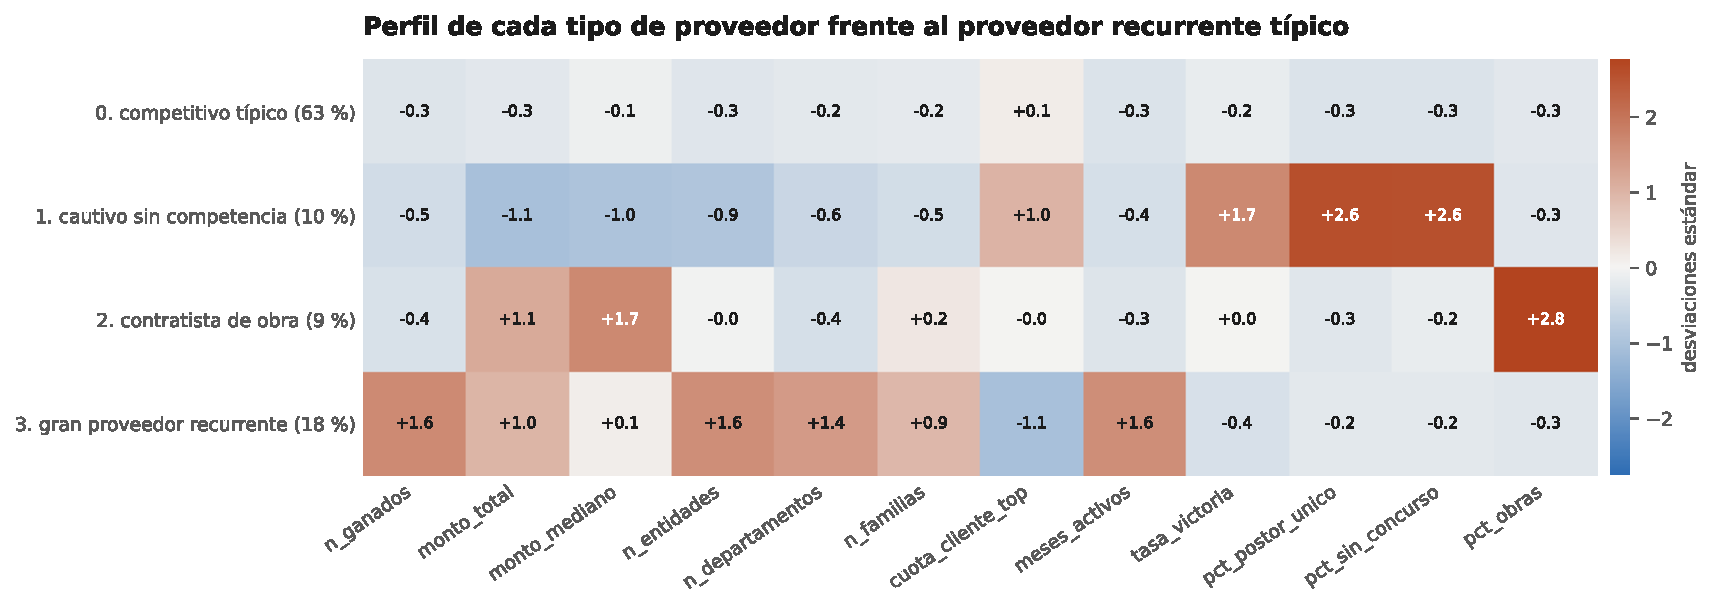
\includegraphics[width=0.92\textwidth]{figs/f11_perfiles_cluster.pdf}
\caption{Perfil de cada cluster en desviaciones estándar respecto del proveedor recurrente típico. El cluster 1 combina dependencia de un cliente con ausencia de competencia.}
\label{fig:perfiles}
\end{figure}

\begin{figure}[h]
\centering
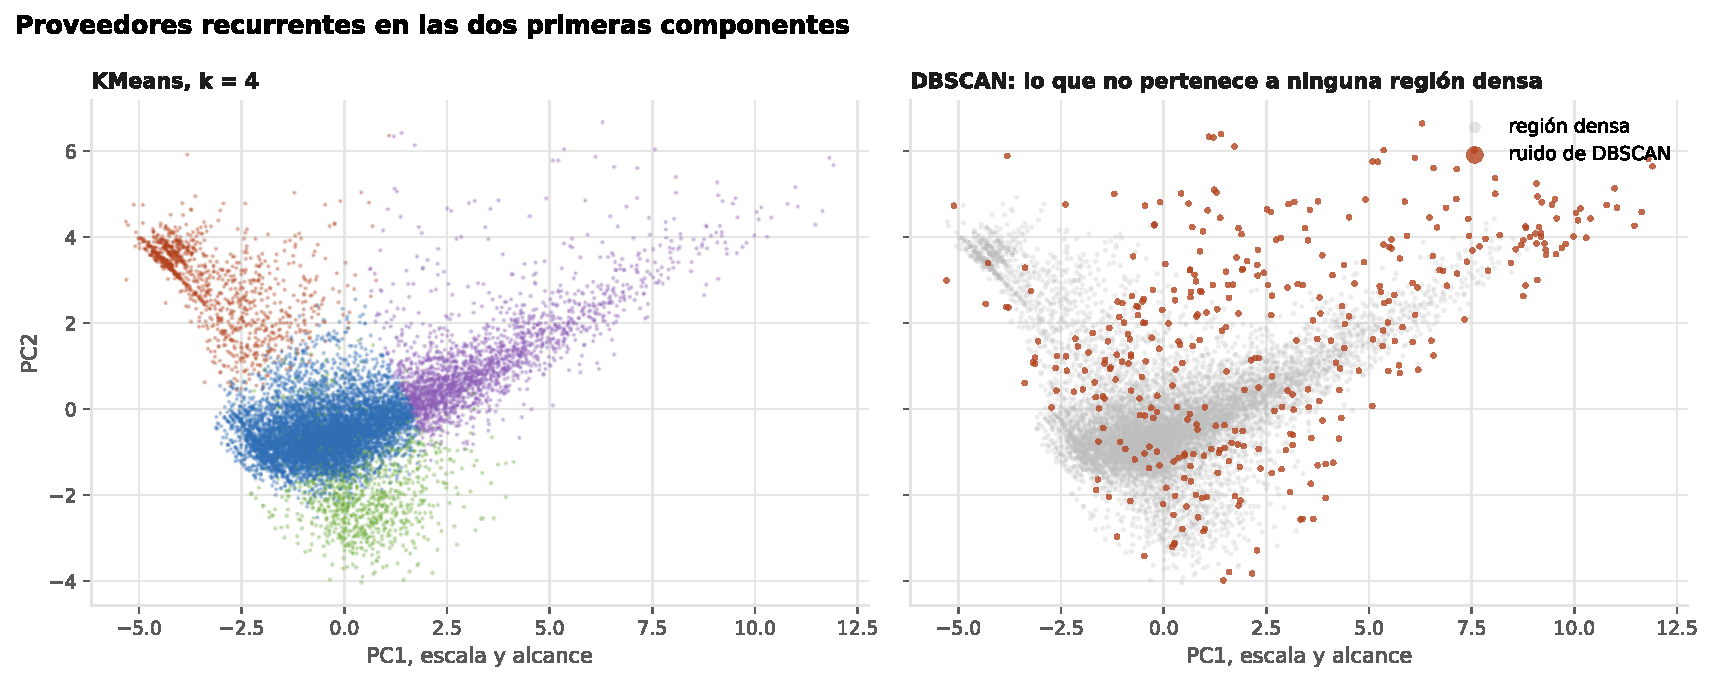
\includegraphics[width=0.95\textwidth]{figs/f14_kmeans_dbscan.pdf}
\caption{Los mismos proveedores en las dos primeras componentes: KMeans corta el continuo en 4 regiones; DBSCAN deja en rojo lo que no pertenece a ninguna región densa.}
\label{fig:kmeans}
\end{figure}

\textbf{Interpretación.} Los cuatro perfiles son el competitivo típico (63 \%), el gran proveedor recurrente (18 \% de proveedores y 49 \% del monto), el contratista de obra (9 \%) y el \textbf{cautivo sin competencia}: 1.260 proveedores que en mediana obtienen el 100 \% de su monto de una sola entidad y ganan sin otro postor el 91 \% de las veces, S/ 1.581 millones. Las anomalías se definen como ruido de DBSCAN unido a distancia extrema al centroide: 260 proveedores, de los cuales 183 lo son por escala (los grandes proveedores nacionales, rareza esperable) y \textbf{77 por competencia o dependencia}, que ganan sin otro postor el 73 \% de las veces. Esa segunda cola es la útil para control.

%==========================================================================
\clearpage
\section*{Propuesta para la Parte III. Sistemas de recomendación}

\textbf{Planteamiento.} Las entidades son los usuarios, los proveedores son los ítems y la señal es implícita, $\log(1+n)$ con $n$ el número de adjudicaciones. La evaluación es temporal: se entrena con 2023 y 2024 y se mide si el sistema anticipa las \textbf{relaciones nuevas de 2025}, con precisión, recall y NDCG en 10 sobre 2.123 entidades. El fin es analítico: medir qué tan esperable es una relación, no sugerir a quién contratar. Proponemos cuatro sistemas, los dos primeros ya prototipados.

\begin{enumerate}
\item \textbf{R1. Híbrido entidad a proveedor.} Suma de puntajes estandarizados por entidad de cuatro señales: vecindario usuario a usuario con coseno ($k=50$, elegido en validación), contenido con TF-IDF de familias CUBSO y departamentos del proveedor, ALS implícito de MLlib (rango 48) y popularidad en el departamento. En el prototipo supera a cada señal sola (figura~\ref{fig:rec}): NDCG de 0,089 frente a 0,067 de la popularidad regional, y la ablación muestra que el vecindario es la señal que más aporta.
\item \textbf{R2. Sustitutos de proveedor.} Vecinos más cercanos en el espacio de factores de ALS. Sin haber visto las familias, el 16 \% de los 10 vecinos comparte la familia principal, frente a 3 \% al azar. Uso: para una entidad que depende de un proveedor cautivo de la Parte II, una lista de invitación a cotizar.
\item \textbf{R3. Entidad a categoría.} El mismo esquema sobre la matriz entidad por familia CUBSO (3,2 \% de densidad, mucho menos dispersa): qué rubros compran entidades parecidas que esta no compra.
\item \textbf{R4. PageRank personalizado como quinta señal.} Caminata aleatoria con reinicio desde cada entidad sobre el grafo bipartito G2 de la Parte IV; el puntaje estacionario de cada proveedor es su cercanía a la entidad por caminos de varios pasos. Conecta las Partes III y IV y se evalúa con la misma partición temporal.
\end{enumerate}

\begin{figure}[h]
\centering
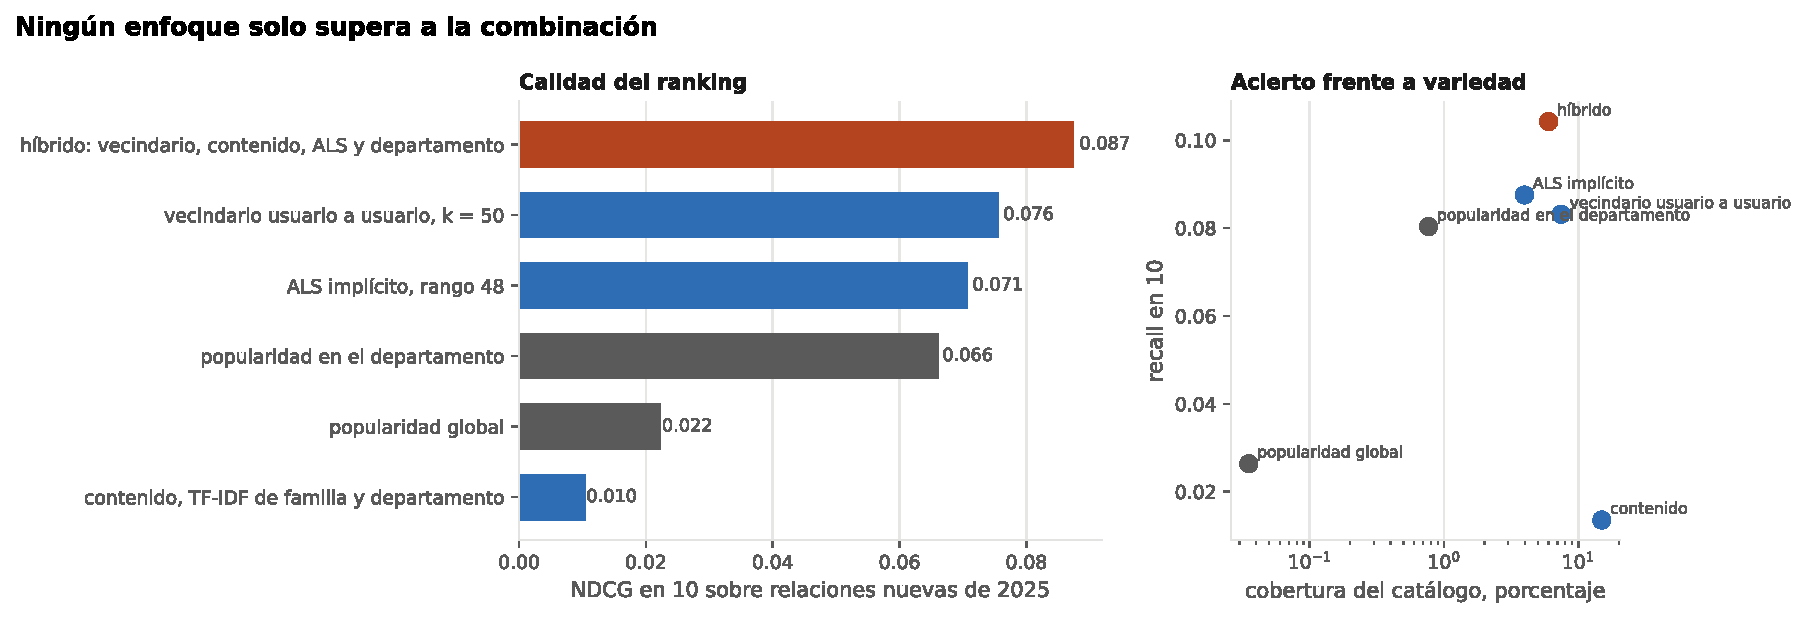
\includegraphics[width=0.8\textwidth]{figs/f17_resultados_recomendacion.pdf}
\caption{Prototipo de R1 sobre relaciones nuevas de 2025. Ningún enfoque solo supera a la combinación.}
\label{fig:rec}
\end{figure}

\textbf{Resultado a reportar con honestidad.} Que una relación sea improbable para el modelo no predice, por sí solo, menos competencia: postor único de 6,2 \% frente a 5,3 \%, $p=0{,}30$. El percentil del modelo se propone para ordenar la revisión dentro de lo que ya es sin concurso o con un solo postor, no como alerta aislada.

%==========================================================================
\clearpage
\section*{Propuesta para la Parte IV. Grafos para PageRank, HITS y grafo KNN}

PageRank calcula $r = \beta M r + \frac{1-\beta}{N}\mathbf{1}$, donde $M$ reparte el rango de cada nodo entre sus aristas salientes y el teletransporte con probabilidad $1-\beta$ evita trampas de araña y callejones sin salida. Su resultado depende de qué significa una arista, por eso proponemos cuatro grafos con preguntas distintas (figura~\ref{fig:grafos}).

\begin{figure}[h]
\centering
\begin{tikzpicture}[
  ent/.style={rectangle,draw=azul,fill=azul!15,minimum size=5mm,inner sep=1pt,font=\scriptsize},
  pro/.style={circle,draw=rojo,fill=rojo!15,minimum size=5mm,inner sep=1pt,font=\scriptsize},
  car/.style={circle,draw=morado,fill=morado!15,minimum size=4mm,inner sep=0pt},
  dir/.style={-{Stealth[length=2mm]},thick},
  titulo/.style={font=\small\bfseries,anchor=west},
  nota/.style={font=\scriptsize,anchor=west,text width=3.6cm,align=left}]
% G1
\begin{scope}
\node[titulo] at (-0.3,1.6) {G1. Coparticipación};
\node[pro] (a) at (0,0.6) {A}; \node[pro] (b) at (1.2,1.0) {B};
\node[pro] (c) at (1.4,0) {C}; \node[pro] (d) at (0.3,-0.5) {D};
\draw[gris,line width=2pt] (a)--(b); \draw[gris,line width=0.6pt] (a)--(d);
\draw[gris,line width=1.2pt] (b)--(c); \draw[gris,line width=0.6pt] (c)--(d);
\node[nota] at (-0.3,-1.25) {no dirigido, peso de Newman; ya construido};
\end{scope}
% G2
\begin{scope}[xshift=4.3cm]
\node[titulo] at (-0.3,1.6) {G2. Bipartito};
\node[ent] (e1) at (0,0.8) {E1}; \node[ent] (e2) at (0,-0.3) {E2};
\node[pro] (p1) at (1.6,1.0) {P1}; \node[pro] (p2) at (1.6,0.25) {P2}; \node[pro] (p3) at (1.6,-0.5) {P3};
\draw[dir,azul] (e1)--(p1); \draw[dir,azul] (e1)--(p2); \draw[dir,azul] (e2)--(p2); \draw[dir,azul] (e2)--(p3);
\node[nota] at (-0.3,-1.25) {entidad a proveedor, peso por monto; HITS};
\end{scope}
% G3
\begin{scope}[xshift=8.6cm]
\node[titulo] at (-0.3,1.6) {G3. Perdedor a ganador};
\node[pro] (x) at (0,0.8) {A}; \node[pro] (y) at (0,-0.3) {B};
\node[pro,fill=rojo!45] (g) at (1.5,0.25) {G}; \node[pro] (z) at (1.5,-0.7) {C};
\draw[dir,rojo] (x)--(g); \draw[dir,rojo] (y)--(g); \draw[dir,rojo] (z)--(g); \draw[dir,rojo] (g) to[bend left=20] (y);
\node[nota] at (-0.3,-1.25) {dirigido, del perdedor al ganador de cada proceso};
\end{scope}
% G4
\begin{scope}[xshift=12.9cm]
\node[titulo] at (-0.3,1.6) {G4. KNN};
\foreach \i/\x/\y in {1/0/0.9,2/0.5/0.4,3/-0.1/0.1,4/1.4/0.8,5/1.8/0.2,6/1.3/-0.4,7/0.4/-0.6}
  \node[car] (k\i) at (\x,\y) {};
\draw[morado] (k1)--(k2) (k2)--(k3) (k1)--(k3) (k4)--(k5) (k5)--(k6) (k4)--(k6) (k3)--(k7) (k2)--(k6);
\node[nota] at (-0.3,-1.25) {$k$ vecinos en el espacio de rasgos o de ALS};
\end{scope}
\end{tikzpicture}
\caption{Los cuatro grafos propuestos. Cuadrados: entidades; círculos rojos: proveedores; morados: proveedores como vectores.}
\label{fig:grafos}
\end{figure}

\begin{enumerate}
\item \textbf{G1. Coparticipación de proveedores} (ya construido, 70.383 nodos). Advertencia que guía la propuesta: en un grafo no dirigido, PageRank sin teletransporte es proporcional al grado ponderado, así que aporta poco sobre contar aristas. Aquí se usará para \textbf{PageRank personalizado} desde los 4.847 pares afines y para las comunidades de la Parte V.
\item \textbf{G2. Bipartito entidad a proveedor} (2.964 entidades y 62.462 proveedores, aristas ponderadas por monto). Es el grafo natural para \textbf{HITS}: los hubs son entidades que contratan a proveedores importantes y las authorities, proveedores contratados por entidades importantes. También alimenta R4.
\item \textbf{G3. Perdedor a ganador} (dirigido, a construir desde participaciones y adjudicaciones). En cada proceso cada postor perdedor apunta al ganador. Aquí PageRank sí dice algo distinto del grado: un proveedor sube si le gana a quienes ganan. Los ciclos cortos, A le gana a B y B le gana a A en procesos alternados, son el patrón de rotación que conviene cruzar con los pares afines. Los procesos con postor único no generan aristas y quedan fuera por diseño.
\item \textbf{G4. Grafo KNN} sobre los 12.062 proveedores recurrentes, con $k=10$ vecinos en las 6 componentes de PCA o en los factores de ALS, simetrizado por unión. Sirve de entrada al clustering espectral y a Node2Vec (Partes V y VI) y permite medir si los clusters de la Parte II, las comunidades y los embeddings convergen (Parte VII).
\end{enumerate}

\begin{table}[h]
\centering\small
\begin{tabularx}{\textwidth}{l l l X}
\toprule
Grafo & Algoritmo & Spark o local & Pregunta \\
\midrule
G1 coparticipación & PageRank personalizado, comunidades & GraphFrames & ¿En qué vecindario de competencia viven los pares afines? \\
G2 bipartito & HITS, PageRank con reinicio (R4) & local, subgrafo & ¿Qué entidades y proveedores son centrales en el mercado? \\
G3 perdedor a ganador & PageRank con sensibilidad a $\beta$ & GraphFrames & ¿Quién domina a quienes compiten? ¿Hay rotación de ganadores? \\
G4 KNN & espectral, Node2Vec & local, 12 mil nodos & ¿Coinciden clusters, comunidades y embeddings? \\
\bottomrule
\end{tabularx}
\caption{Resumen de la propuesta de grafos. La sensibilidad al factor de amortiguamiento se medirá con $\beta$ entre 0,5 y 0,95 comparando el solapamiento de los 100 primeros.}
\end{table}

\end{document}
